\chapter{Discourse in longer texts: Leveraging coreference}
\label{ch:longertexts1}
This chapter is the first of two that examines how to incorporate discourse from longer texts into computational models. In this chapter, I explore cohesion devices (through coreference) for the NLP task of information extraction.

Work in this chapter has been published in \newcite{Ferracane:2016}.

\section{Chapter Overview}
Performing systematic reviews is a critical yet manual, labor-intensive step in evidence-based medicine. Automating systematic reviews is an active area of research, requiring innovations in machine learning and computational linguistics. We examine how coreference resolution can aid in identifying the arms of a study, an often overlooked piece of information needed to synthesize the results in a systematic review. A classification model\footnote{\tt https://github.com/elisaF/extractGroups} that performs better with the coreference features supports the intuition that coreference is able to capture the discourse salience of arms. We note that control arms do not benefit as much from these features. 


\begin{table}[h]
\begin{adjustbox}{center}
\begin{tabular}{p{10.5cm}}
\hline
{\small Randomised controlled trial with 12 month intervention. Change in body mass index (BMI) standard deviation score (SDS) over 12 months with assessment 18 months after the start of the intervention. Using the last available data on all participants (n=106), those in the $\underbrace{\hbox{Mandometer group}}_{\text{arm1}}$ had significantly lower mean BMI SDS at 12 months compared with $\underbrace{\hbox{standard care}}_{\text{arm2}}$. The mean meal size in the $\underbrace{\hbox{Mandometer group}}_{\text{arm1}}$ fell by 45 g. Those in the Mandometer group also had greater improvement in concentration of high density lipoprotein cholesterol.}\\\hline
  \end{tabular}
  \end{adjustbox}
  \caption{Excerpt from medical abstract illustrating the discourse salience of the intervention arm, \textit{arm1}, where the control arm is \textit{arm2} (note that not all mentions of the arms are annotated in the gold data, as discussed in section \ref{subsec:errors}).}
  \label{tab:1}
\end{table}
\begin{table}[h]
\begin{adjustbox}{center}
\begin{tabular}{p{10.5cm}}
\hline
{\small Randomised controlled trial with 
	\begingroup
      \color{blue}
	    $\overbrace{\color{black}\hbox{12 month intervention}}^{\text{chain1}}$
       \endgroup
    . Change in body mass index (BMI) standard deviation score (SDS) over 12 months with assessment 18 months after the start of
    \begingroup
      \color{blue}
     $\overbrace{\color{black}\hbox{the intervention}}^{\text{chain1}}$
     \endgroup
. Using the last available data on all participants (n=106), 
    \begingroup
      \color{violet}
     		$\overbrace{\color{black}\hbox{those in 
           \begingroup
            \color{red}
             $\overbrace{\color{black}\hbox{the $\underbrace{\color{black}\hbox{Mandometer group}}_{\color{black}\text{arm1}}$}}^{\text{chain3}}$
             \endgroup
             }}^{\text{chain2}}$ 
       \endgroup
had significantly lower mean BMI SDS at 12 months compared with $\underbrace{\hbox{standard care}}_{\text{arm2}}$. The mean meal size in 
	\begingroup
      \color{red}
    $\overbrace{\color{black}\hbox{the $\underbrace{\color{black}\hbox{Mandometer group}}_{\color{black}\text{arm1}}$}}^{\text{chain3}}$
    \endgroup
fell by 45 g. 
    \begingroup
      \color{violet}
    $\overbrace{\color{black}\hbox{Those in 
        \begingroup
          \color{red}
    				$\overbrace{\color{black}\hbox{the Mandometer group}}^{\text{chain3}}$
         \endgroup
        }}^{\text{chain2}}$
  \endgroup
also had greater improvement in concentration of high density lipoprotein cholesterol.}\\\hline
  \end{tabular}
  \end{adjustbox}
  \caption{Medical abstract with annotated arms and coreference chains. The chains were automatically determined as described in section \ref{subsec:coref-features}. All phrases with the same chain label are judged to co-refer.}
  \label{tab:2}
\end{table} 
\section{Introduction}

Evidence-based medicine (EBM) is a paradigm that seeks to inform medical practitioners of the optimal treatment, based on the totality of the available evidence (i.e., the results of all relevant clinical trials). To this end, teams of medical experts often conduct \textit{systematic reviews}, which synthesize all published medical literature pertaining to a specific clinical question. The first step in a systematic review is to formulate the research question to be investigated, and then find all of the relevant citations. Abstracts and then full texts are screened to exclude irrelevant trials. Once a set of trials pertinent to the research question are identified (typically 10-20 trials), key pieces of information are extracted from each trial. This information generally consists of the patient Population under study, the Intervention(s) being tested, the Comparison and the Outcomes (abbreviated as PICO). Results from all identified trials are typically statistically combined via meta-analysis to produce an aggregated result. 
%The outcome numbers across all trials are statistically combined to produce a single synthesized result, which is then published in the final report of the systematic review. 


Producing systematic reviews is a time-consuming, largely manual process. This is exacerbated by the rapidly growing evidence base: PubMed\footnote{\tt publicly available resource for accessing medical references and abstracts https://www.ncbi.nlm.nih.gov/pubmed/} contains 800,000+ publications on clinical trials in humans \cite{Wallace:2013}, and on average reports of 75 new trials are published daily.  A single systematic review can take over a year to produce -- at which point it risks becoming outdated. Therefore, automating evidence synthesis poses an enormous yet enticing challenge for automation. %The sheer volume and increasing rate of publication, together with the thousands of specialized person-hours expended in reviews, pose an enormous yet enticing challenge for automation.

A crucial step towards automating synthesis is identifying the \textit{arms}, or groups, in trials. A clinical trial consists of one control arm, and one or more  intervention arms. For example, a study comparing the efficacy of aspirin versus a placebo would consist of two arms: those taking \textit{aspirin} (the intervention group), and those taking the \textit{placebo} (the control group). Previous work has mostly focused on identifying the PICO elements. However, the PICO elements alone are insufficient to convey the design of the study, a key piece of evidence necessary in the downstream task of data synthesis and analysis. Thus, the present study focuses on improving the automated identification of arms. We observed that arms are often salient in the discourse of the abstract, in that they corefer more often than other tokens. This study is exploratory work that focuses on investigating the effectiveness of using coreference features for identifying arms. % bcw: I think this is sufficient; we may make another note below regarding state-of-the-art, etc
%We do not attempt to achieve state-of-the-art results, but instead seek to understand whether and how coreference may help in labeling arms. 

The remainder of this chapter is organized as follows. We motivate the choice of coreference features for arm identification. We then examine prior work in identifying the arms in medical texts, and how coreference resolution has been applied to the medical field. Next, we present an experiment to classify whether tokens in annotated medical abstracts are part of an arm. We propose features that take advantage of the discourse salience of arms, and we discuss the results with and without the coreference features.

\section{Motivation}
Identifying the arms is not a simple information extraction task. The arms in a study consist of one control group, and one or more intervention groups. Often, the control group is never explicitly mentioned in the abstract. In the following excerpt, only the intervention arm is mentioned:
\vspace{-.5em}

\begin{table}[H] 
\begin{tabular}{p{7cm}}
\small{\textit{To determine whether modifying eating behaviour with use of\uline{ a feedback device} facilitates weight loss in obese adolescents.}}
\end{tabular}
\end{table}
\vspace{-1.2em}
An arm in a study is typically a noun phrase (NP), where this NP is repeated, either verbatim or anaphorically, throughout the abstract. An example of the discourse salience of arms in a medical abstract is in Table \ref{tab:1}. The intervention arm, \textit{Mandometer group}, is repeated several times verbatim throughout the abstract.

Given this recurring linguistic pattern in medical abstracts, we investigated the use of \textit{coreference resolution} to help identify arms. The goal of coreference resolution is to determine which mentions in a text refer to the same entity. A referring expression, or \textit{mention}, is the natural language expression used by discourse participants to refer to entities. Two or more mentions that refer to the same entity are coreferent, and together form a \textit{coreference chain}. An anaphor and its antecedent (or cataphor and its postcedent) will form a coreference chain. Mentions can be indefinite noun phrases, definite noun phrases, proper names and pronouns, where clinical trial abstracts contain mostly NP's. Using an off-the-shelf coreference tool (to be discussed in more detail in section \ref{subsec:coref-features}) yields the mentions and coreference chains illustrated in Table \ref{tab:2}.

Note that the token \textit{intervention}, which is not part of an arm, appears at most 2 times within a single coreference chain, whereas \textit{Mandometer}, part of the experimental arm, appears 3 times. Further, \textit{intervention} is found only in 1 chain, whereas \textit{Mandometer} appears in 2 chains. More generally, we hypothesize a token forming part of an arm is more salient in two ways: (i) an arm token appears more often within a single coreference chain, and (ii) an arm token appears more frequently across different chains (within the same abstract). These observations motivate the coreference features presented in section \ref{subsec:features}. In Table \ref{tab:2}, \textit{“standard care”} is not a member of any chains. More generally, we can expect salience to help more with intervention arms than control.\footnote{Cases of joint coreference such as \textit{all participants} referring to both arms in the example abstract are not addressed in this work, but pose an interesting problem for identifying PICO elements such as population and outcome.}

\section{Related work}
\subsection{Automated Identification of Arms}

Previous work has identified PICO elements either at the word or sentence level. Most research has extracted information from medical abstracts, although some studies have used the full text of the articles \cite{DeBruijn:2008,Zhao:2012,Wallace:2016}. One of the seminal studies in PICO extraction \cite{Demner:2007} collapsed intervention and comparator, where interventions were short noun phrases based largely on recognition of semantic types (mapped to UMLS concepts) and a few manually constructed rules. The intervention/comparator extractor returned a list of all the interventions under study, and the extractor was evaluated at the sentence level. However, it is important to distinguish between experimental and control treatments as the bias for the experimental group must be accounted for in the data synthesis step \cite{Lumley:2002}. 

Beyond PICO, \newcite{DeBruijn:2008} extracted data from full-text articles based on the CONSORT Plus Guideline,\footnote{\tt http://rctbank.ucsf.edu/home/cplus} a list of required, recommended and optional items to include in a systematic review compiled by medical experts. The study found that one of the most difficult items to identify was the experimental treatment, which varied widely beyond just drug names. Elsewhere, \newcite{Chung:2009} identified interventions as a coordinating structure in a single sentence, and found the major weakness in this approach was parsing errors when identifying the boundaries of the conjuncts. And \newcite{Summerscales:2011} focused on the downstream task of calculating the absolute risk reduction (ARR), identifying the number of bad outcomes for the control and experimental treatment groups, along with the sizes of both treatment groups. This study found outcomes hardest to detect because of their variability, but also had an overall poor recall partly because coreference was not taken into account.

%Some studies stand out for going beyond the PICO elements. \newcite{deBruijn2008} extracted data from full-text articles based on the CONSORT Plus Guideline \footnote{\tt http://rctbank.ucsf.edu/home/cplus}, a list of required, recommended and optional items to include in a systematic review compiled by medical experts. The study found that one of the most difficult items to identify was the experimental treatment, which varied widely beyond just drug names.


Most recently, \newcite{Trenta:2015} proposed a novel approach for identifying the arms and PICO elements that does not rely on a first stage of sentence classification, but instead classifies each token directly, followed by an inference process to constrain the labels to more accurate results. As with previous studies, outcome results were the hardest because they are more variable. A significant limitation of this study is that the abstracts were limited to two-arm trials, and in a specific domain.

\subsection{Automated Coreference Resolution}
\label{subsec:coref}

% bcw: I would say we could cut pretty dramatically here if we really need the space; I think it's beyond the scope of the current work to provide in-depth history (or even really a brief history) of co-ref -- probably sufficient to say 'this is a long-standing problem, go read XXX' 
Coreference resolution is a long-studied task that remains a challenging problem. Most recent work on coreference resolution builds mainly on one of four models. 
\begin{itemize}
\item The first and most widely-used approach is the \textit{mention-pair} model \cite{Soon:2001,Ng:2002}. A classifier first identifies all the pairs of mentions which are coreferent. These pairs are then grouped into coreferent chains by clustering techniques such as closest-first \cite{Soon:2001} or best-first \cite{Ng:2002,Ng:2002b}. In closest-first, you link to the closest preceding mention, whereas in best-first, you choose the likeliest one. Common features in these models include distance between the two mentions, syntactic features (e.g.,  POS tags), semantic features (e.g., named entity type), lexical features (e.g., head word of the mention), and string matching.
\item  The \textit{mention-ranking} model \cite{Denis:2008}, reframes the task as a ranking function rather than a classification function, ranking all the candidate antecedents of a mention to determine which candidate antecedent is the most probable.
\item The \textit{entity-centric} model makes use of entity-level information, focusing on features of mention \textit{clusters}, and not just pairs \cite{Raghunathan:2010}. The coreference clusters are built up incrementally, using information from  partially-completed coreference chains to guide later decisions. Features include whether a mention head word matches any of the head words in the antecedent cluster.
 \item The \textit{antecedent tree model} \cite{Yu:2009} builds a graph from a document, where the nodes are the mentions and arcs are the links between mention pairs that are coreferent candidates. The coreference chains are then modeled as latent trees in the graph.
\end{itemize}
Constraints are imposed on these models for improved results, such as enforcing a transitive closure to guarantee you end up with legal assignments \cite{Finkel:2008}. For example, if \textit{John Smith} is coreferent with \textit{Smith}, and \textit{Smith} with \textit{Jane Smith}, then it should not follow that \textit{John Smith} and \textit{Jane Smith} are coreferent. Other work has shown that joint models improve performance. \newcite{Denis:2007} recognized that anaphoricity (whether an entity is the first mention) and coreference should be treated as a joint task since one informs the other. \newcite{Durrett:2014} models coreference together with named entity recognition and linking named entities to Wikipedia entities. Combinations of these models have also yielded improved results, such as \newcite{Clark:2015} stacking \textit{mention-pair} and \textit{entity-centric} systems (which the current work uses as its off-the-shelf coreference resolver).

Many coreference resolvers exploit deeper linguistic knowledge, beyond the features mentioned above. \newcite{Chowdhury:2013} eliminated less-informative training instances prior to model training by creating a list of criteria based on semantic and syntactic intuitions such as a mismatch in semantic types. \newcite{Peng:2015} created predicate schemas to constrain inference, such as two predicates with a semantically shared argument. \newcite{Yang:2015} used semantic role labeling to link the time and locations for event mentions, and for verbal mentions they linked their participants. More recently, \newcite{Kilicoglu:2016} focused on sortal anaphoras which they found to commonly occur in biomedical literature, resolving anaphors that carry a specific semantic type, or sort, such as \textit{these drugs}.  Many of these studies take advantage of linguistic resources such as WordNet\footnote{\tt http://wordnet.princeton.edu} and FrameNet\footnote{\tt https://framenet.icsi.berkeley.edu}.

In the medical area, coreference resolution has been most closely studied for analyzing clinical narrative text such as that found in Electronic Health Records (EHRs), and biomolecular studies. In fact, there have been corpora (i2b2/VA Corpus\cite{Uzuner:2012}, GENIA Event Corpus\cite{Kim:2008}) and shared tasks (SemEval-2015 shared task on “Analysis of Clinical Text” (Task 14)\cite{Elhadad:2015}, BioNLP’09 shared task\cite{Kim:2009}, ShARe/CLEF eHealth 2013 Evaluation Lab Task 1\cite{Pradhan:2013}) created specifically to advance this area. Given that resources such as FrameNet and WordNet are based mostly on news (e.g. British National Corpus, U.S. newswire), a large number of resources have been created to aid in natural language processing of medical texts. By far the largest and most complex is the Unified Medical Language System (UMLS)\footnote{\tt https://www.nlm.nih.gov/research/umls/}, consisting of three main components:  Metathesaurus with terms and codes from many vocabularies (including CPT, ICD-10-CM, MeSH, RxNorm, and SNOMED CT), Semantic Network with semantic types and semantic relations, and the SPECIALIST Lexicon, which contains syntactic, morphological and orthographic information on terms, along with NLP tools such as POS tagger and word sense disambiguator. Other tools include MetaMap\footnote{\tt https://metamap.nlm.nih.gov}, a tool for recognizing UMLS concepts, DrugBank\footnote{\tt http://www.drugbank.ca}, a database of drug names, BANNER\footnote{\tt http://banner.sourceforge.net}, a named entity recognizer for biomedical texts, BioText for identifying entities and relations in bioscience texts, and BioFrameNet\footnote{\tt http://biotext.berkeley.edu}, an extension of FrameNet for molecular biology (and BioWordNet\cite{Poprat:2008} was a failed attempt at extending WordNet also to the biomolecular field). However, when applied to clinical trial texts, these tools prove useful mainly for identifying only medical terms and drug names, and thus more linguistically-motivated resources are still lacking for clinical trial texts.

In the area of clinical narratives, \newcite{Raghavan:2012} took advantage of the temporal features present in these texts to help determine whether two medical concepts corefer with each other. Their 2014 paper \cite{Raghavan:2014} expanded on this idea to identify medical events spanning across narratives, such as admission notes, medical reports, and discharge notes. \newcite{Yoshikawa:2011} exploited coreference information for extracting event-argument relations from biomedical texts in the Genia Event Corpus. \newcite{Jindal:2013} used very specific domain knowledge to resolve coreference in clinical narratives, such as creating a specific discourse model (i.e. a single patient, several doctors and a few family members) to resolve entities of type "person".  Despite the active interest in coreference resolution, there has been much less research investigating its application to clinical trial texts. Most of the literature that does exist is applied to the bio-medical field, focusing more on full-text articles \cite{Gasperin:2008,Huang:2010,Kilicoglu:2016} than on abstracts \cite{Castano:2002,Yang:2004}. To the best of the authors' knowledge, there have been no papers using coreference features to identify arms in clinical trial abstracts. 

\section{Experiment}

The goal of this experiment is to explore empirically whether incorporating coreference features improves the performance of a classifier for arm identification, as compared to a baseline model without coref features (note that we do not aim to necessarily achieve state-of-the-art results on this task). The task of the classifier is to label a token as either part of an arm or not.

\subsection{The corpus}

The corpus\footnote{\scriptsize {\tt https://github.com/rlsummerscales/bibm2011corpus}} consists of 263 abstracts from the British Medical Journal (BMJ) annotated with the experimental and control groups (and other PICO elements) by \newcite{Summerscales:2013}. The BMJ requires structured input, and the number of sections varies with some abstracts only containing a few sections such as BACKGROUND, METHODS, FINDINGS and INTERPRETATION. These structured abstracts usually consist of short phrases and incomplete sentences. 

\begin{table}[h]
  \begin{tabular}{l||l}
      \hline
      Number of documents & 263 \\
      Number of tokens & 63,488 \\
      Number of [abstract, token] pairs & 35,650 \\
      Average no. tokens per document & 241 \\
      Positive labels & 5,757 (9\%) \\\hline
  \end{tabular}
  \caption{Corpus statistics}
  \label{tab:3}
\end{table}
\vspace{-1em}

\subsection{Experimental setup}

Sentences were tokenized, lower-cased and stop words were removed . Each token was paired with its abstract to form an \textit{[abstract, token]} pair to uniquely correlate the token with the medical abstract where it appeared (e.g. \textit{[abstract\_3, "intervention"], [abstract\_129, "intervention"]}). A binary classifier was implemented to label each token as belonging to an arm or not (scikit-learn implementation of Support Vector Machine, \newcite{scikit-learn}). Due to the imbalance of classes (9\% positive), the class weights in the model were adjusted to be inversely proportional to the class frequencies in the corpus. We performed five-fold cross validation.

\begin{table*}[ht]
  \centering
    \begin{tabular}{l|l|l|l}
        \hline
        Model & Precision (var) & Recall (var)& F1 (var)\\\hline\hline
        baseline & 12.9 (2.7e-04) & 88.6 (5.6e-04) & 22.5 (6.2e-04)\\
        coref & \textbf{19.7} (7.5e-04) & 82.7 (8.4e-04) & \textbf{31.8} (14.4e-04)\\
        tfidf2 & 18.2 (9.75e-04) & \textbf{89.2} (7.81e-04) & 30.3 (1.47e-03) \\\hline
    \end{tabular}
    \caption{Results averaged across 5-folds on the two models with their variances in parentheses.}
  \label{tab:5}
\end{table*}

\begin{table}[h]
  \begin{tabular}{l|l|l|l}
      \hline
      Feature & Mean & Range & Variance \\\hline\hline
      b-o-w & 1.78 & 1-24 & 2.71\\
      drugbank & 0.09 & 0-1 & 0.08\\
      tf-idf & 6.06 & 1-141.1 & 42.67\\
      coref max\_counts & 0.14 & 0-15 & 0.31\\
      coref num\_chains & 0.10 & 0-6 & 0.11\\\hline
  \end{tabular}
  \caption{Feature statistics}
  \label{tab:4}
  %\vspace{-.5em}
\end{table}

\subsection{Features}
\label{subsec:features}
The following features, summarized in Table \ref{tab:4}, were used in the machine learning algorithm.

\noindent {\bf bag-of-words} The number of times the token occurs within its medical abstract (i.e., the count of \textit{[abstract, token]} pairs for the given token and abstract). As evident in Table \ref{tab:4}, abstracts can be quite repetitive in their vocabulary, but on average a token appears only a couple of times within the same abstract.

\vspace{.25em}

\noindent {\bf drugbank} Whether the token exists in the DrugBank database version 4.3\footnote{\scriptsize {\tt http://www.drugbank.ca/system/downloads/4.3/drugbank.xml.zip}}. The clinical trials often compare the efficacy of different drugs, such that intervention arms would contain drug names. However, note from Table \ref{tab:4} that most words are not drugs, keeping in mind that interventions also consist of therapies, behavior changes and other non-drug-related treatments.

\vspace{.25em}
% bcw: if hurting for space, can remove TF-IDF formulas, as pretty standard
\noindent {\bf tf-idf:} Term frequency-inverse document frequency for term $t$ in document $d$ for corpus $D$:
\vspace{-.5em}
\begin{equation}\label{tfidf}
tf\text{-}idf_{t,d} = tf_{t,d} * (idf_{t,D} + 1),
\end{equation}
where:
\vspace{-1.5em}
\begin{equation*}
\begin{aligned}
tf_{t,d}& =f_{t, d}\\
idf_{t, D}& =  \log \frac{|D|}{|\{d \in D: t \in d\}|}\\
\end{aligned}
\end{equation*}

One is added in the equation \eqref{tfidf} so that terms with zero idf (those that occur in all documents of a training set) are not entirely ignored. The goal of this metric is to capture how informative a word is. For example, the token \textit{mandometer} (an arm) from the abstract in Table \ref{tab:2} has a tf-idf measure of 26.29, whereas \textit{intervention} (not an arm) has a value of 3.7. On average, the tokens are slightly more informative than common words such as \textit{intervention}.

\subsection*{coreference:}\label{subsec:coref-features} The Coreference Resolution annotator packaged in Stanford Core NLP 3.0\footnote{\scriptsize {\tt http://nlp.stanford.edu/software/stanford-corenlp-full-2015-12-09.zip}} (a model that stacks \textit{mention-pair} and \textit{entity-centric} systems) is used to calculate the maximum number of times the token occurs in a single coreference chain within the same medical abstract (\textbf{max\_counts}) and the number of chains the token appears in the same medical abstract (\textbf{num\_chains}). This tool was chosen because it is publicly available and yields state-of-the-art results on the 2012 CoNLL data set. The coreference features aim to capture the discourse salience of arms in medical abstracts. As mentioned before, the (max\_counts, num\_chains) values for \textit{mandometer} are (3,2), but for \textit{intervention} are (2,1). Note from Table \ref{tab:4} that although a token can occur very frequently in a single chain (\textit{max\_counts}) and across many chains (\textit{max\_chains}), a token on average is not part of a chain at all. This observed statistic lends weight to the use of coreference features as a measure of salience. Previous work has employed other features such as dependency trees and other predicate argument structures to capture this discourse salience. \newcite{Summerscales:2013} implemented a form of post-hoc coreference resolution as a way to cluster labeled words into groups, for example into a control group versus an intervention group. However, the present study uses the coreference features at the front end to detect the mentions, and is presently not concerned with differentiating among the different arms. 

\section{Evaluation}
Table \ref{tab:5} summarizes the evaluation scores. The results of the classifier are evaluated against the spans of text that were annotated as arms, following \newcite{Summerscales:2013}. Because an arm consists of several contiguous words (e.g. \textit{mandometer group}), we want to ensure the classifier is able to correctly label the more informative words in that span (\textit{mandometer} vs.  \textit{group}). A labeled group of words is considered a match for an annotated group if they consist of the same set of words, ignoring \textit{had, group(s)}, and \textit{arm}. For example, a labeled span of \textit{mandometer} for the annotated span \textit{mandometer group} is a true positive. On the other hand, a labeled span of only \textit{group} is a false positive. Although the scores are relatively low for both models, we emphasize the goal of this experiment is not to achieve state-of-the-art results but to investigate the viability of salience for arm identification. Further, we are being strict in our evaluation, compared to prior work (e.g., \newcite{Summerscales:2013} ). % bcw: I **think** this is true!? I recall he is quite lax with counting things as agreeing?

\subsection{Baseline}

The \textbf{baseline} model includes the features for how many times a token appears in a single abstract (\textbf{b-o-w}), whether the token exists in the DrugBank (\textbf{drugbank}), and the term-frequency inverse-document-frequency measure for the token (\textbf{tf-idf}).

\subsection{With Coreference}
The \textbf{coref} model additionally includes the maximum number of times the token appears in a single coreference chain for a given abstract (\textbf{max\_counts}), and the number of coreference chains the tokens appears in for a given abstract (\textbf{num\_chains}).

\subsection{Error Analysis}\label{subsec:errors}

\begin{figure}
\centering
\begin{subfigure}{.5\textwidth}
  \centering
  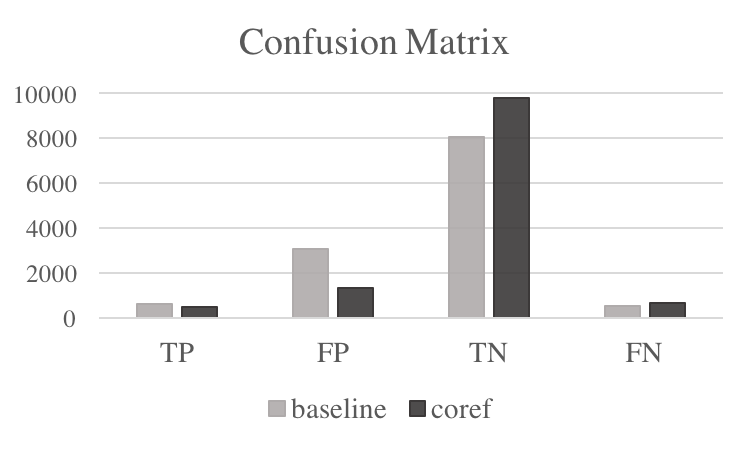
\includegraphics[width=1\linewidth]{plots/longer1_confusion_matrix_bar_chart.png}
  \caption{raw counts}
  \label{fig:conf_matrix_unnormalized}
\end{subfigure}%
\begin{subfigure}{.5\textwidth}
  \centering
  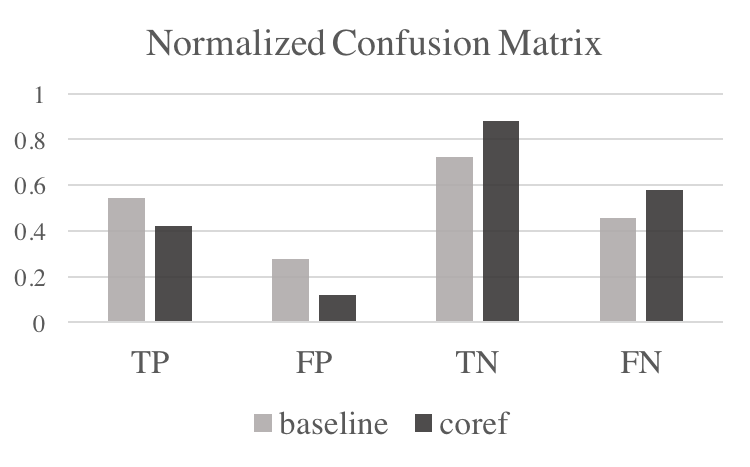
\includegraphics[width=1\linewidth]{plots/longer1_confusion_matrix_norm_bar_chart.png}
  \caption{normalized}
  \label{fig:conf_matrix_normalized}
\end{subfigure}
\caption{The confusion matrices with raw counts (a) and normalized counts (b) for the baseline and coref models.}
\label{fig:conf_matrix}
\end{figure}

The coref model performed better than the baseline model in almost all the metrics: precision (improved 6.8 points) and F1 (+9.3). Additionally, these improvements are consistent across all the cross-validation runs, as illustrated in Figure \ref{fig:f1}. Adding the coreference features lowers recall by 5.9 points. To understand the results in more detail, we compare the confusion matrices of the two models. The raw counts in Figure \ref{fig:conf_matrix_unnormalized} illustrate the class imbalance of the data, giving the impression that a false positive is more likely than a false negative. The normalized confusion matrices in Figure \ref{fig:conf_matrix_normalized} show that false negatives are a higher percentage of the errors than false positives, so that the positive class is the harder one to label. 

\begin{figure}[t]
\centering
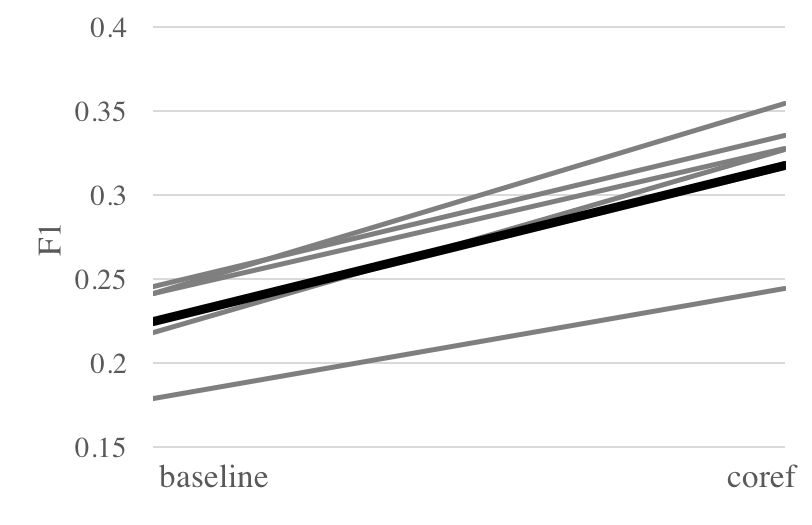
\includegraphics[scale=0.5]{plots/longer1_f1_variance.png}
\vspace{-0.5em}
\caption{F1 score across the 5 runs in gray, with mean in the thick black line. The lines connect results in the baseline model to results of the the same folds in the coref model.}
\label{fig:f1}
\vspace{-.5em}
\end{figure}

Given that false negatives are the most common errors across both models, we analyze their occurrences first. The control arm is the most susceptible to this type of error, as it is not as salient in the discourse as the experimental arms. The control words are typically drawn from a finite and small vocabulary (e.g. \textit{control, placebo, sham, standard}), so their tf-idf scores are usually low. The false negative rate worsens in the coref model partly because it places more weight on discourse salience, and control arms are often not part of a coreference chain, compared with experimental arms. We refer back to the abstract presented in Table \ref{tab:1}. A small ablation study was conducted to determine that the b-o-w feature is able to correctly label \textit{standard} (count=4) as part of an arm. With the coreference features, the word is no longer labeled as an arm, as it does not appear in any coreference chain.

Next, we analyze the false positives across both models. Given that all the features (except drugbank) in both models are aimed at extracting salient words, they also pick out other relevant PICO information. For example, both models incorrectly label \textit{knee} as part of an arm in the following abstract, where each of these mentions is, in fact, annotated as part of an \textit{outcome}:

\begin{table}[h] 
\begin{tabular}{p{7cm}}
{\small \textit{...reduce the incidence of \uline{knee} and ankle injuries in young people participating in sports. The rate of acute injuries to the \uline{knee} or ankle. A structured programme of warm-up exercises can prevent \uline{knee} and ankle injuries...}}
\end{tabular}
\vspace{-1.8em}
\end{table}
\vspace{3 mm}  
Another issue with false positives is that the gold data is not comprehensively annotated. Note that in Table \ref{tab:2}, the annotator failed to label the third occurrence of \textit{mandometer} as an arm, although both models attempt to classify it as such. However, striving for a thoroughly annotated data set is not realistic, and so the models should be more robust to these gaps and inconsistencies. The false positive rate improves in the coref model partly because the coreference features prove to be a better measure of discourse salience for the intervention arms. As noted earlier, repetition in medical abstracts is not limited to the words describing the arm. For example, in the abstract from Table \ref{tab:1}, the baseline model incorrectly labels the high-frequency tokens \textit{eating, months} and \textit{mean} as parts of an arm. The coref model instead correctly labels these as negative, given that they do not occur in a coreference chain. 

Finally, we note that the coreference features help in grouping together words with  conflicting tf-idf measures. In the abstract from Table \ref{tab:1}, the baseline model correctly labels \textit{mandometer} (tf-idf=26.3), but misses \textit{group} (tf-idf=4.2). However, the coref model correctly labels the entire span \textit{mandometer group} as an arm, because both of these tokens appear together in a mention and have the same coreference features.

\section{Chapter Summary}
We introduced a new approach to identify the arms in a clinical trial abstract by creating coreference features aimed at capturing the discourse salience of arms. The coreference features were shown to help in classifying a word as part of an arm, confirming the intuition that mentions of arms throughout the abstract often corefer. However, we note this pattern holds more for the experimental than control arms. The error analysis also revealed that arms are not the only concepts that are coreferent: other PICO elements such as the outcome often have the same features. This observation could motivate a model that jointly labels these PICO elements along with the arms, since one would inform the other. There are several other recurring linguistic patterns yet to be explored that could further aid in arm identification, such as apposition:
\vspace{-.7em}
\begin{table}[h] 
\begin{tabular}{p{7cm}}
{\small\textit{A computerised device, \uline{Mandometer}, providing real time feedback...}}
\end{tabular}
\vspace{-.5em}
\end{table}

and paraphrasing:
\vspace{-.7em}
\begin{table}[h] 
\begin{tabular}{p{7cm}}
{\small\textit{..half were \uline{produced  automatically  with  a  larger  volume  of  material}...The \uline{larger  booklets  produced  automatically} were...}}
\end{tabular}
\vspace{-.5em}
\end{table}

Another avenue of research is to investigate how these linguistic features pattern across abstracts in the same review. For example, finding the paraphrases across all abstracts that study the same treatment (as defined in a systematic review) could yield finer-grained information on the language used to describe that intervention. To compensate for the inconsistent and small number of annotations, label propagation might be used to retrieve clusters of relations and find the structure in the data.

As noted earlier, the present study focused on the effect of salience on arm identification. In a future study, we plan to implement \newcite{Summerscales:2013} as a strong baseline (which achieved an F-score of 0.69) to understand whether coreference can still yield improved results when compared to a model that nears state-of-the-art performance.



